\documentclass[11pt,english,compress]{beamer}
\usepackage[utf8]{inputenc}
\usepackage{verbatim}
\usepackage{eurosym}
\usepackage{ stmaryrd }

\useoutertheme{smoothbars}
\useinnertheme[shadow=true]{rounded}
\usecolortheme{orchid}
\usecolortheme{whale}
\title{Nouveau}
\subtitle{Recap, on-going and future work}
\author{Martin Peres, Lucas Stach \& the Nouveau community}
\institute{Ph.D. student at LaBRI, B.Eng. student at HfTL}
%\logo{\includegraphics[width=1.5cm]{imgs/ensib.jpg}}

\AtBeginSection[]{
  \begin{frame}{Summary}
  \small \tableofcontents[currentsection, hideothersubsections]
  \end{frame} 
}

\begin{document}

\setbeamertemplate{navigation symbols}{}

\begin{frame}
	\titlepage
\end{frame}

\section{The Nouveau community at FOSDEM}
	\begin{frame}
			\begin{block}{Your host for the next hour}
				\begin{itemize}
					\item Martin Peres (mupuf)
					\item Maarten Lankhorst (mlankhorst)
					\item Lucas Stach (lynxeye)
				\end{itemize}
			\end{block}
			\begin{block}{Also attending}
				\begin{itemize}
					\item Emil Velikov (xexaxo)
					\item Francisco Jerez (curro)
					\item Roy Spliet (rspliet)
				\end{itemize}
			\end{block}
	\end{frame}

\section{History}
	\begin{frame}
		\begin{block}{History: NVIDIA -- a new hope}
			\begin{itemize}
				\item 1998(?): NVIDIA releases a Linux open-source 2D-only driver(nv)
				\item 1998: Obfuscation commit (release only pre-processed source)
			\end{itemize}
		\end{block}
	\end{frame}

	\begin{frame}
		\begin{block}{}
			After we already finalized XFree86-3.3.3 NVIDIA forced The XFree86 Project
			to replace the sources we had with sources that were partly run through the
			C preprocessor in order to remove some of the names that NVIDIA thought
			might give away IP from NVIDIA. This resulted in unreadable and unmaintainable
			code.
		\end{block}

		\begin{block}{}
			The XFree86 Project is strongly opposed to such obfuscated code. We do not
			regard this as free software according to our standards. Due to the extremely
			late date of this decision from NVIDIA we decided to include the code as
			offered by NVIDIA. We are considering to remove support for the later NVIDIA
			chips in a future release, though.
		\end{block}

		 Xfree86, commit message from 11/18/98
% http://cvsweb.xfree86.org/cvsweb/xc/programs/Xserver/hw/xfree86/vga256/drivers/nv/Attic/README.RIVATNT.diff?r1=1.1.2.2&r2=1.1.2.3&hideattic=0&only_with_tag=xf-3_3_3
% http://cvsweb.xfree86.org/cvsweb/xc/programs/Xserver/hw/xfree86/vga256/drivers/nv/Attic/nv3driver.c.diff?r1=1.1.2.5&r2=1.1.2.6&hideattic=0&only_with_tag=xf-3_3_3
	\end{frame}

	\begin{frame}
		\begin{block}{History: The open-source strikes back}
			\begin{itemize}
				\item 2005: Stephane Marchesin improves nv and works on 3D
				\begin{itemize}
					\item Project named Nouveau after an unfortunate automatic spelling correction
					\item Back-port nv updates to Nouveau
				\end{itemize}
				\item 2008: Open Arena runs on nv40
				\item 2009: KMS driver based on TTM
				\item 2010: Merged in Linux 2.6.33
				\item 2010: Nv is deprecated by NVIDIA, say ``use VESA''.
			\end{itemize}
		\end{block}
	\end{frame}

	\begin{frame}
		\begin{block}{History: The return of the Jedi}
			``It's so hard to write a graphics driver that open-sourcing it
			would not help [...] In addition, customers aren't asking for opensource drivers.''\\
			Andrew Fear, NVIDIA software product manager, April 2006
			%http://news.cnet.com/New-Linux-look-fuels-old-debate/2100-7344_3-6061491.html
		\end{block}
	\end{frame}

\section{Architecture}
	\subsection{Short hardware introduction}
		\begin{frame}
			\begin{block}{Chipset families}
				\begin{itemize}
					\item NV03: RIVA 128
					\item NV04: RIVA TNT/TNT2
					\item NV10: Geforce2/4 MX
					\item NV20: Geforce 3, Geforce 4 Ti
					\item NV30: Geforce FX
					\item NV40: Geforce 6/7 (the first real family) 
					\item NV50: Geforce 8/9/100/200/300 (the biggest family)
					\item NVC0: Geforce 400/500, AKA Fermi
					\item NVD9: Half-Kepler chipset
				\end{itemize}
			\end{block}
		\end{frame}

		% XXX: give short overview over hw engines (microcode slide only here for reference)
		\begin{frame}
			\begin{block}{Hardware Introduction}
				\begin{itemize}
					\item NVIDIA GPUs consists of "objects"
					\item command submission by DMA buffers
					\item GPU can accesss system memory through the aperture
					\item NV50 features a full blown virtual memory system
				\end{itemize}
			\end{block}
			\begin{block}{important engines}
				\begin{itemize}
					\item PFIFO: main command fetching engine
					\item PCRTC/PDISPLAY: display scanout engines
					\item PGRAPH: main graphics object AKA OpenGL cast into silicon
					\item PMPEG: video acceleration found on older cards (not much use today)
					\item PVDEC/PPPP: modern video decoding engines %mlankhorst: please elaborate and remove comment
				\end{itemize}
			\end{block}
		\end{frame}

	\subsection{Components}
		\begin{frame}
			\begin{block}{The 4 parts of Nouveau}
				\begin{itemize}
					\item Linux Kernelmodule
					\item libdrm-nouveau
					\item DDX: xf86-video-nouveau
					\item Mesa3D drivers:
						\begin{itemize}
							\item nouveau-vieux
							\item nvfx
							\item nv50
							\item nvc0
						\end{itemize}
				\end{itemize}
			\end{block}
		\end{frame}

		\begin{frame}
			\begin{block}{Linux kernel module Nouveau}
				\begin{itemize}
					\item Resource management
						\begin{itemize}
							\item GPU Channels
							\item Memory Management
						\end{itemize}
					\item Command-submission
					\item Kernel Mode Setting
					\item Power Management
				\end{itemize}
			\end{block}
		\end{frame}

		% some deeper insights about pm here XXX: please update
		\begin{frame}
			\begin{block}{Power management}
 				\begin{itemize}
					\item Parsing power-management table from the vbios
					\item Temperature management: thermal calibration + fan management
					\item Setting the clocks: changes the performance level
					\item Other: clock gating, PCIE downclocking, DAC reclocking
				\end{itemize}
			\end{block}

			\begin{block}{current state}
				\begin{itemize}
					\item nvc0: setting engines clocks (mostly)
					\item nv40-d9: memory timings (almost ready)
					\item nv30-c0: some kind of support to reclock (unreliable)
					\item nv50-a3: reliable clock changes (almost)
					\item fan management: toogle (todo), pwm (done), i2c (WIP)
					\item performance counters (initial work on nv40-c0)
				\end{itemize}
			\end{block}
		\end{frame}

		\begin{frame}
			\begin{block}{WIP}
				\begin{itemize}
					\item nva3-d9: setting memory clocks
					\item nv50-a3: fixing bugs
					\item nv50-d9: getting stable reclocking
					\item AGP/PCIE, clock gating: reverse engineering
					\item Fan: temperature-based management (toogle, pwm and i2c)
					\item perform infrastructure, dynamic reclocking
				\end{itemize}
			\end{block}

			\begin{center}
				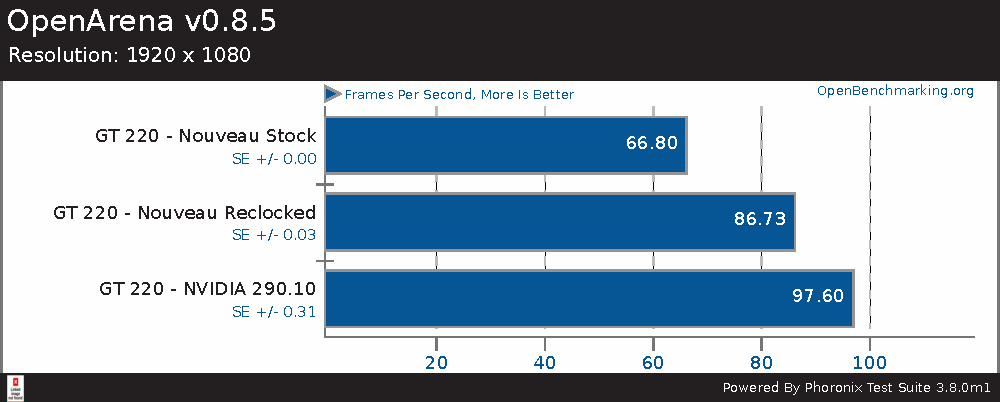
\includegraphics[height=3cm]{imgs/gt220_openarena_bench.pdf}
			\end{center}
		\end{frame}

		\begin{frame}
			\begin{block}{libdrm-nouveau}
				\begin{itemize}
					\item buffer management
						\begin{itemize}
							\item everything is a buffer!
						\end{itemize}
					\item wraps around the IOCTL interface
				\end{itemize}
			\end{block}
			\begin{block}{work in progress}
				\begin{itemize}
					\item currently rewritten
					\item designed with nv40 class hardware in mind
					\item pushbuffer replay
				\end{itemize}
			\end{block}
		\end{frame}

		\begin{frame}
			\begin{block}{DDX -- xf86-video-nouveau}
				\begin{itemize}
					\item EXA (2D acceleration) 
					\item X-Video
					\item supports full range of GPUs (NV04 - NVD9)
					\item makes use of all engines for acceleration (including 3D engine)
				\end{itemize}
			\end{block}
		\end{frame}

		\begin{frame}
			\begin{block}{Mesa3D: drivers for 3D and more}
				\begin{itemize}
					\item two different approaches here: Classic and Gallium3D
					\item nouveau-vieux: classic Mesa3D driver for NV04,NV1x,NV2x
						\begin{itemize}
							\item only supports fixed function OpenGL
						\end{itemize}
					\item Gallium pipe-driver
						\begin{itemize}
							\item nvfx
							\item nv50
							\item nvc0
						\end{itemize}
				\end{itemize}
			\end{block}
		\end{frame}

		\begin{frame}
			\begin{center}
				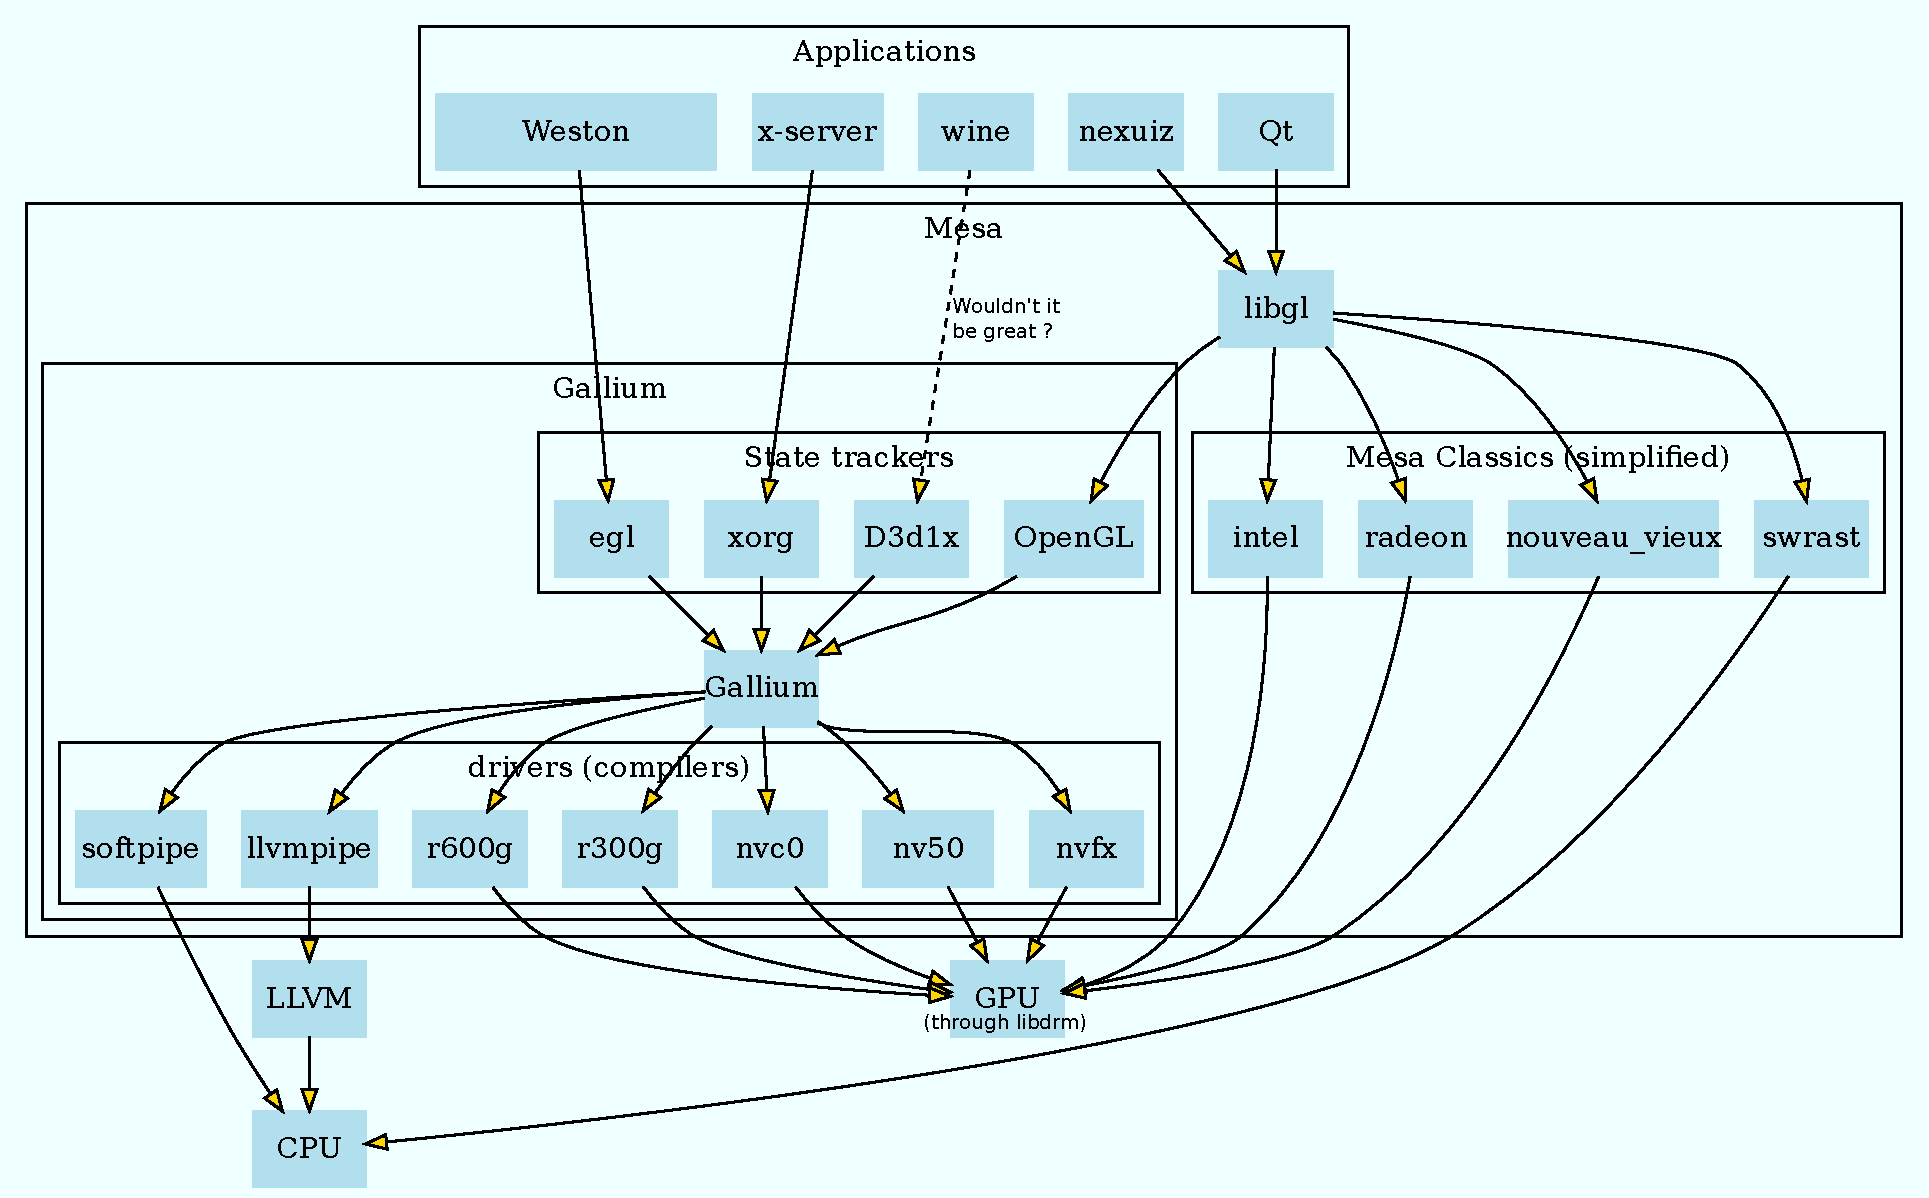
\includegraphics[height=7cm]{imgs/mesa.pdf}
			\end{center}
		\end{frame}

		\begin{frame}
			\begin{block}{nvfx}
				\begin{itemize}
					\item Gallium driver for NV3x,4x class GPUs
					\item one of the first gallium drivers
					\item created by merging separate nv30 and nv40 drivers
					\item accumulated much old cruft
					\item no maintainer for over one year
				\end{itemize}
			\end{block}
			\begin{block}{work in progress}
				\begin{itemize}
					\item will hopefully be soon replaced by rewritten driver
				\end{itemize}
			\end{block}
		\end{frame}
		\begin{frame}
			\begin{block}{nv50}
				\begin{itemize}
					\item Gallium driver for NV50 class GPUs
					\item current codebase was formed by adapting nvc0
					\item maybe first free software driver to allow hardware OpenCL
				\end{itemize}
			\end{block}
			\begin{block}{work in progress}
				\begin{itemize}
					\item merge reworked shader compiler
					\item implement remaining OpenGL 3 features
					\item merge OpenCL work
				\end{itemize}
			\end{block}
		\end{frame}
		\begin{frame}
			\begin{block}{nvc0}
				\begin{itemize}
					\item nvc0: Gallium driver for NVC0 class GPUs
					\item one of the first drivers to support OpenGL 3
				\end{itemize}
			\end{block}
			\begin{block}{work in progress}
				\begin{itemize}
					\item working towards features in DX11 and OGL3+
				\end{itemize}
			\end{block}
		\end{frame}
		\begin{frame}
			\begin{block}{OpenCL}
				\begin{itemize}
					\item WIP by Francisco Jerez
					\item sponsored by the X.org EVOC
					\item very experimental
					\item don't miss curro's presentation (18:00-19:00)
				\end{itemize}
			\end{block}

			\begin{block}{d3d1x}
				\begin{itemize}
					\item Direct 3D 10/11 on Gallium
					\item ``works'' only on nouveau, still a bit hackish
					\item developped by nv50/c0's maintainer: Christoph Bumiller
					\item Unigine Heaven runs ont it when using a modified version of wine
				\end{itemize}
			\end{block}
		\end{frame}

		% XXX: maybe get one slide for video decoding in here
		\begin{frame}
			\begin{block}{Video decoding}
				\begin{itemize}
					\item What's the point?
				\end{itemize}
			\end{block}

			\begin{block}{PMPEG}
				\begin{itemize}
					\item found by luck
					\item does mpeg1/2 decoding
				\end{itemize}
			\end{block}

			\begin{block}{VPx}
				\begin{itemize}
					\item used by nvidia
					\item decode every kind of flux
				\end{itemize}
			\end{block}
		\end{frame}

		\begin{frame}
			\begin{center}
				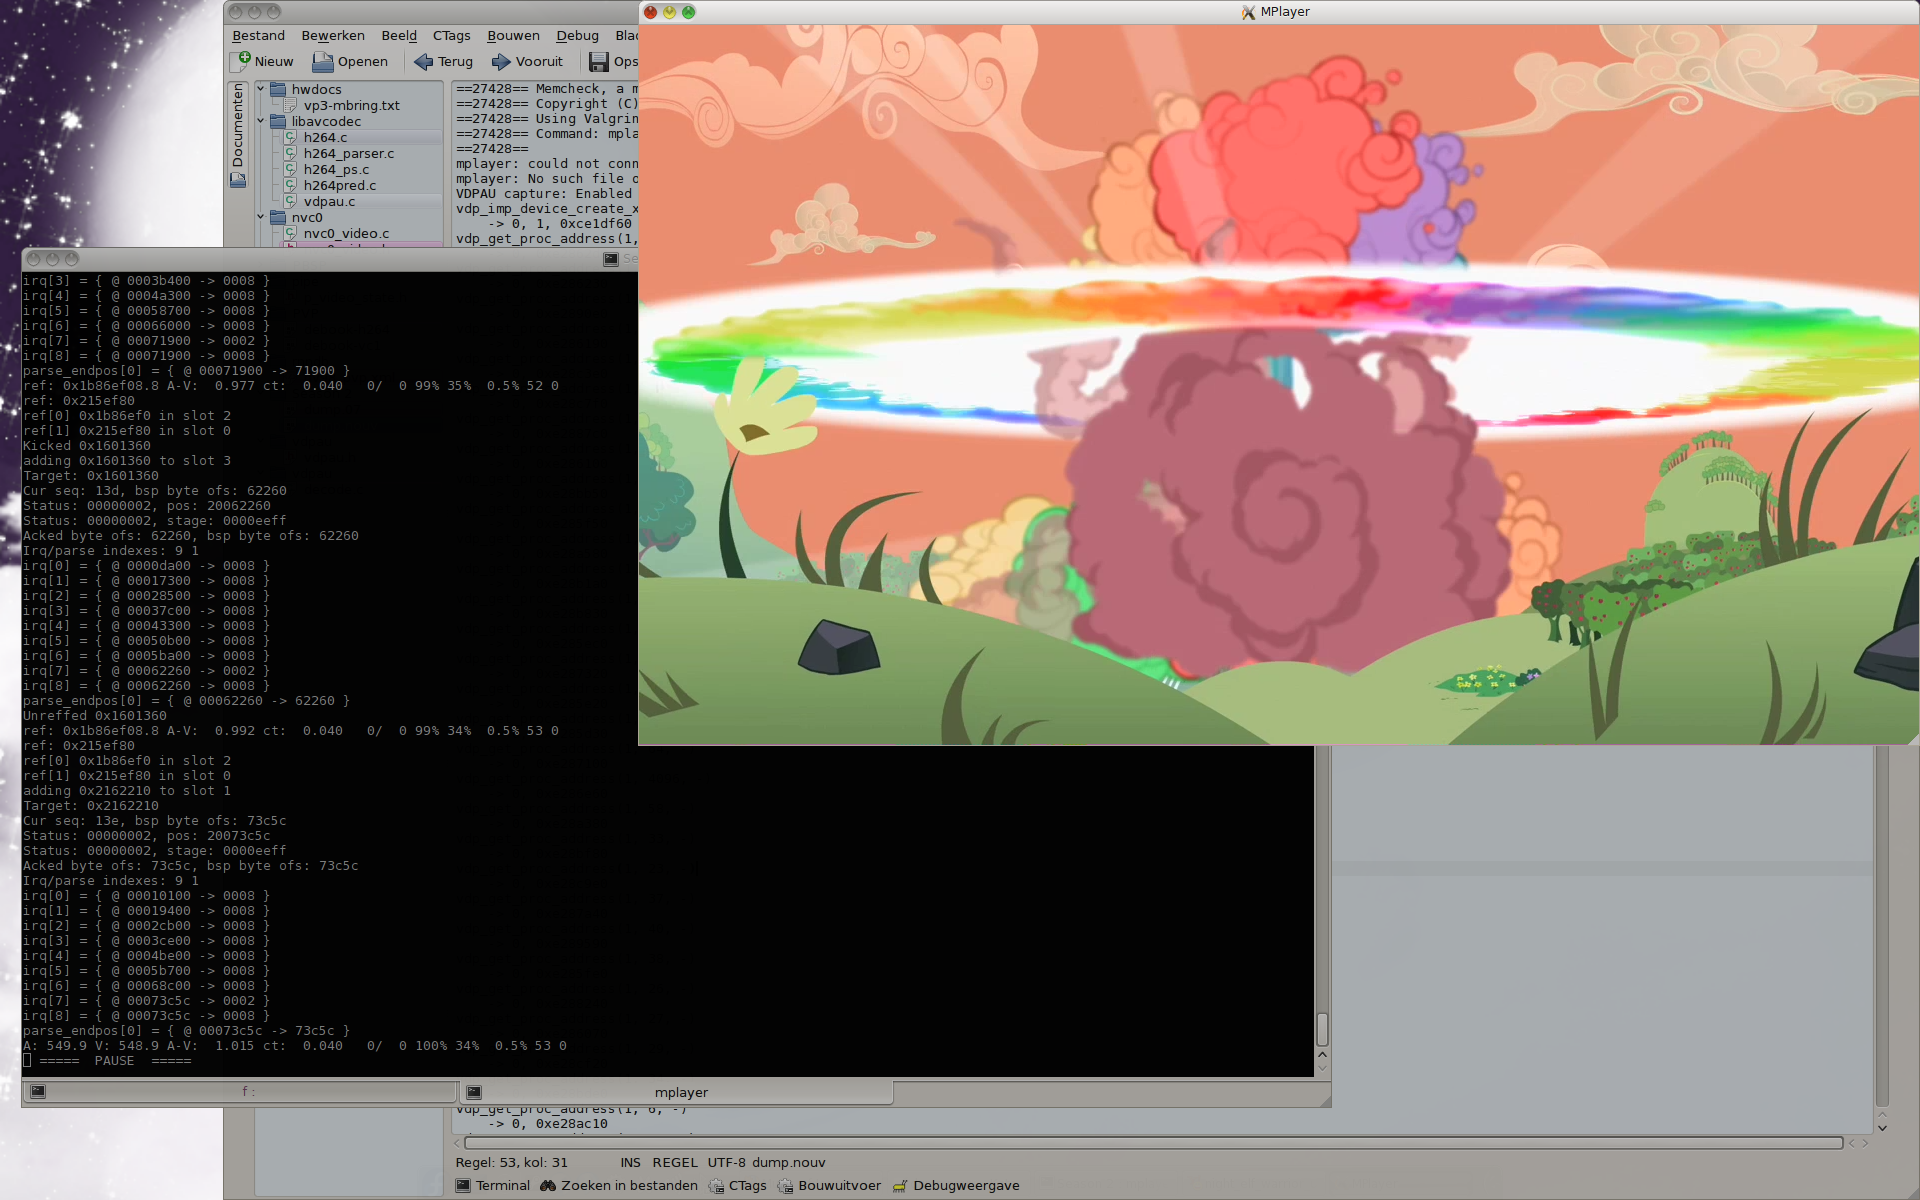
\includegraphics[height=7cm]{imgs/h264_vp_decoded2.png}
			\end{center}
		\end{frame}

\section{Conclusion}
		\begin{frame}
			\begin{block}{Why Nouveau?}
				\begin{itemize}
					\item support old cards unsupported by the blob ($<$ nv40)
					\item support new features (KMS, Xrandr, wayland, d3d1x)
					\item plug \& play support, no need to install and maintain the blob
					\item for the fun!
				\end{itemize}
			\end{block}
		\end{frame}

\section{Demos}
	\begin{frame}
		\begin{block}{MPEG1/2 video decoding}
			\begin{itemize}
				\item using MPlayer
				\item Kernel-side: done
				\item Mesa: merged in 8.0
			\end{itemize}
		\end{block}

		\begin{block}{reclocking and opengl}
			\begin{itemize}
				\item performance improvements in OpenArena/Nexuiz
				\item performance improvements in xvmc
				\item dynamic reclocking (load-based reclocking)!
			\end{itemize}
		\end{block}
	\end{frame}
\end{document}
